

離島架橋の介入効果

<要約>

本稿では離島架橋が離島人口に与える影響を島別パネルデータを用いて推定した.介入の時系列的かつ横断的な異質性を考慮した
Fully Saturated TWFE
モデルを利用し,得られた推定値を平滑化することで介入効果のパターンを明確にした.その結果,離島架橋の介入効果は介入数年前から正の方向に作用し,徐々にその効果を高め,人口減少を抑制する力を持つことを明らかにした.

<キーワード> 離島,人口,離島架橋,因果推論,ATT,Two-way Fixed
Effects,Dynamic TWFE,Fully Saturated
TWFE,階層ベイズモデル,状態空間モデル

\hypertarget{ux306fux3058ux3081ux306b}{%
\section{\texorpdfstring{\(1.\)
はじめに}{1. はじめに}}\label{ux306fux3058ux3081ux306b}}

離島架橋とは,本土と離島,又は離島同士を結ぶために架けられる橋のことを指す.日本は
6,852
の島嶼により構成される島国であり,本州,北海道,四国,九州,沖縄本島を除く
6,847 島が離島である(国土交通省 国土政策局 離島振興課
2022).このうち,離島振興法による離島振興対策実施地域に含まれる有人離島は
254 島であるが,1955 年から 2015 年までの間に,全国の人口が約 4
割増加する一方で,これらの有人離島の人口は約 6 割減少している.

このような離島の人口減少に対し,離島架橋は有効な対策となりうるのか.離島架橋は,離島の交通インフラとして経済活動の活性化や生活環境の向上に寄与する可能性がある一方で,ストロー効果を引き起こし人口流出を招く可能性も指摘されている.本研究は,離島架橋が離島人口に与える影響を定量的に明らかにすることを目的とする.

続いて先行研究のレビューを行う.

橋に肯定的な意見を持つ論文として,沖山ら \((2001)\),宮内ら \((2003)\)
等が挙げられる.一方でやや否定的なものは,寺井ら \((1998)\),湯本ら
\((2002)\),黒田 \((2003)\),猪原ら \((2015)\)
が挙げられる.その他,山崎ら \((2007)\)
は架橋されていない中で人口が増加した島を分析しており,重松 \((2022)\)
は人口変化の要因分析を行っているが架橋の効果に対してはどちらとも言えない立場である.

まず肯定的な意見を持つ論文からレビューを行う.沖山ら \((2001)\)
は,佐賀県加部島における農業を事例として離島の基幹産業に与える架橋政策の影響に関する研究を行っている.架橋前は農道の発達が悪く,生産性が極めて低かったが,架橋後は,土地改良,農道の整備,農業の機械化を促進させ,生産性を向上させた上に,パイプラインによって農業用水が確保されたことで水不足が解消され,陸路によって安定した出荷が出来るようになった.宮内ら
\((2003)\) は 沖縄県浜比嘉島を対象に \(1997\)
年に架橋した浜比嘉大橋による人口増加の影響を分析している.米軍向け野菜供給地として指定されていたが,台湾からの安価な野菜輸入により需要が減少し,農業が衰退.農民層が労働需要が盛んな地域に移住したため激しい人口流出を経験した.浜比嘉大橋完成により,沖縄島と道路で結ばれた島には島外から
U
ターンを中心とする転入者が相次いだ.浜比嘉島は年通勤可能架橋島であるため,人口麺の架橋効果が大きいとのことであった.離島の人口流出対策として,交通インフラ整備が有効であることを示唆している.

一方でやや否定的な意見を持つ論文として,寺井ら \((1998)\)
は,芸予諸島において,本四架橋を契機とした島嶼整備のあり方に関する研究を行っている.架橋の問題点は,渡船業者が大きな影響を受けたり,島らしさを体現する観光資源を衰退に導いているということだと述べられている.湯本ら
\((2002)\) では有人離島 \(423\) 島農地離島振興法対象の \(288\)
離島を対象に,離島の類型化と人口増減要因に関する基礎的分析を行っている.離島の類型化は
\(4\) 側面,自然特性 \(12\) 指標,生活環境 \(16\) 指標,産業形態 \(19\)
指標,離島の側からのアピールポイント \(11\)
指標から主成分分析によって行われた.特に生活環境に関する指標は交通,生活,保健,教育,余暇等からなる指標を用いており,ある主成分は正の方向に「空港が利用可能」
「船の大きさ」 「中学校あり」.負の方向に「他から送水」 「最大就航回数」
「本土から行ける」が付置されていることから,「核的 ――
枝的」軸と解釈されている.人口増加に対しては,自然特性が圧倒的に大きな影響力を持ち,長期人口増及び社会増には本土へのアクセス等よりも島での快適な暮らしが効果的であると述べられている.黒田
\((2003)\)
は架橋されている周防大島と架橋されていない小豆島を比較して,架橋の影響を分析している.架橋が行われる前は両者の傾向は変わらないが,架橋後は周防大島の方が減少の度合いが大きいと述べられている.猪原ら
\((2015)\)
は,明石海峡大橋を事例として空間経済学に基づくストロー効果の検証を行っている.ストロー効果を,交通インフラの整備等による
\(2\)
地域間輸送費の低下により,一方の地域の出荷額が他方の地域と比べて相対的に減少することと定義して分析しており,兵庫県では市場拡大効果が優勢で出荷額増加が観察された一方,徳島県では競争拡大効果が優勢で出荷額減少が見られた.明石海峡大橋開通後,徳島県の中小店舗が経済的影響を強く受けたとしている.

その他,山崎ら \((2007)\) は \(1970\) 年から \(30\)
年にわたって人口増加を続けた特異な離島である兵庫県姫路市家島町に属する防勢島を研究している.その島に橋はないが,防勢島は自然増が社会減を上回る形で人口が増加しているが,その要因は,養殖への産業構造の変化と埋め立てによる住宅用地の確保,新宅分けという慣行にあると述べられている.

どちらとも言えない立場として,重松 \((2022)\) は \(1980\) から \(2020\)
年の \(272\)
島を分析対象として,離島の人口変化の要因分析を行っている.被説明変数には人口比率や合計特殊出生率,死亡率,転入率,転出率.説明変数には本土からの距離や平均気温等の自然地域特性,各産業の従業員数等の島内雇用,架橋の有無等の行政の取組,年代別等の人口を用いて重回帰分析をしている.架橋の有無を示すダミー変数のパラメータの推定値に関しては,\(2020\)
年の人口変化率に対して \(1.25\) と正の影響を与えているが,\(2010\)
年の転入率に対しては \(-0.52\) ,\(2010\) 年の転出率に対しては \(-0.40\)
と負の影響を与えている.\(2010\)
年時点では転出超過が起きるストロー効果が発生しているが,\(2020\)
年ではストロー効果を起こしていないと述べられている.

これらの先行研究は,個別の離島における架橋の影響を詳細に分析しているものや,複数の離島を用いて類型化や要因分析を行っているものがあるが,離島架橋に注目してその平均的な効果を定量的に検証した研究は存在しない.本研究は,複数の離島における架橋前後のデータを用いて,離島架橋の動的な介入効果を推定する点に新規性がある.

また本研究は,インフラ投資の政策効果を実証的に検証することで,離島振興政策の立案に示唆を与える点で社会的意義を持つ.離島架橋が人口維持に有効であれば,政府は離島架橋への財政支出を通じて離島の経済活動の活性化や生活環境の向上を図ることができる.一方,効果が限定的であれば,政府は他の政策手段を検討することで,有限な資源のより効果的な配分を目指すことができる.

本稿の構成は以下の通りである.第 \(2\) 章では分析手法を説明する.第
\(3\) 章では分析結果を示し,第 \(4\)
章では実際の人口データと照らし合わせながら考察を述べ,第 \(5\)
章ではまとめを行う.

\hypertarget{ux5206ux6790ux624bux6cd5}{%
\section{\texorpdfstring{\(2.\)
分析手法}{2. 分析手法}}\label{ux5206ux6790ux624bux6cd5}}

本章では,まず使用するデータの説明をし,次に平行トレンドの仮定の検証をした後,\(3\)
つのモデルを紹介する.最後に \(\text{Student-t}\)
分布を用いたロバスト推定を説明する.

\hypertarget{ux4f7fux7528ux30c7ux30fcux30bf}{%
\subsection{\texorpdfstring{\(2.1\)
使用データ}{2.1 使用データ}}\label{ux4f7fux7528ux30c7ux30fcux30bf}}

本稿の実証分析では,島別のアンバランスドパネルデータを使用する.分析対象の島は瀬戸内地域を中心に中国・四国地方から選択した
\(78\) 島であり,介入群 \(33\) 島,対照群 \(45\) 島とする.
介入群の選定基準は,架橋前の人口データが入手可能かどうかであり,対照群の選定基準は,本土もしくは他の島からの距離が
\(1991m\) 以内であるかどうかである.\(1991m\)
はギネスブックに掲載されていた元世界最長の吊り橋である明石海峡大橋の全長であり,これよりも距離が長い場合は,技術の進歩を加味しても,いずれ架橋される可能性は低い.また離れすぎていると人口動態が異なる場合があるため,対照群として適さないと判断した.
分析期間は最長で \(1960\) 年から \(2020\) 年,最短で \(1995\) 年から
\(2020\) 年までとし,国勢調査を基本とした \(5\) 年毎のデータを用いる.
人口データは主に国勢調査から取得\footnote{都道府県市区町村というウェブサイトから小地域区分を取得し,合計することで人口データを得た.}し,足りない部分は離島統計年報や地方自治体のウェブサイトから補完した.
橋の開通年は地方自治体のウェブサイトを参照し,その島で最初に開通した橋の開通年を採用した.地方自治体のウェブサイトが見つからない場合は,Wikipedia
「日本の離島架橋」を参照した\footnote{地方自治体の情報と Wikipedia
  の情報が異なる場合は前者を採用.}.

\begin{longtable}[]{@{}ll@{}}
\toprule
項目 & 出典\tabularnewline
\midrule
\endhead
人口 & 国勢調査離島統計年報地方自治体のウェブサイト等\tabularnewline
橋の開通年 & 地方自治体のウェブサイト等Wikipedia
「日本の離島架橋」\tabularnewline
\bottomrule
\end{longtable}

注: 筆者作成

また,各変数の基本統計量は以下の通りである.人口は分散が大きく,最小値と最大値は
\(1\)
万倍以上の差がある.平均に対して標準偏差が非常に大きいため,正規性を仮定することが難しい.一方対数人口は安定した分散を持ち,正規性を仮定しやすい.その上,人口の変動を変化率で捉える事ができるため,被説明変数には対数人口を用いる.
介入変数は,架橋年以降で \(1\) を取るダミー変数である.平均は \(0.26\)
であり,全てのデータポイント中 \(26\%\) が介入後のデータとして扱われる.
介入年は \(1970\) 年から \(2016\) 年までの範囲であり,平均は \(1989.56\)
年である. 経過年数は介入年からの相対年数であり,介入年を
\(0\),介入前を負の値,介入後を正の値で表す.平均は \(5.88\)
年であり,最小値は \(-46\) 年,最大値は \(50\) 年である.

\begin{longtable}[]{@{}cccccc@{}}
\toprule
項目 & 平均 & 標準偏差 & 最小 & 中央 & 最大\tabularnewline
\midrule
\endhead
人口 & \(2084.47\) & \(5664.25\) & \(4\) & \(232.50\) &
\(44819\)\tabularnewline
対数人口 & \(5.70\) & \(2.02\) & \(1.39\) & \(5.45\) &
\(10.71\)\tabularnewline
介入変数 & \(0.26\) & \(0.44\) & \(0\) & \(0\) & \(1\)\tabularnewline
介入年 & \(1989.56\) & \(12.48\) & \(1970\) & \(1988\) &
\(2016\)\tabularnewline
経過年数 & \(5.88\) & \(20.04\) & \(-46\) & \(6\) &
\(50\)\tabularnewline
\bottomrule
\end{longtable}

注: 筆者作成

\hypertarget{ux5e73ux884cux30c8ux30ecux30f3ux30c9ux306eux4eeeux5b9aux3068ux691cux8a3c}{%
\subsection{\texorpdfstring{\(2.2\)
平行トレンドの仮定と検証}{2.2 平行トレンドの仮定と検証}}\label{ux5e73ux884cux30c8ux30ecux30f3ux30c9ux306eux4eeeux5b9aux3068ux691cux8a3c}}

本稿では差の差分析 (DID) を基本としたモデルを使用する.DID
における重要な識別仮定の一つである平行トレンドの仮定は,反実仮想として,介入がなかった場合の介入群のトレンドが対照群のトレンドと平行であったという想定を指す.本節では,この仮定の妥当性を定量的に検証する.

\hypertarget{ux4ecbux5165ux524dux306eux30c8ux30ecux30f3ux30c9ux5206ux6790}{%
\subsubsection{\texorpdfstring{\(2.2.1\)
介入前のトレンド分析}{2.2.1 介入前のトレンド分析}}\label{ux4ecbux5165ux524dux306eux30c8ux30ecux30f3ux30c9ux5206ux6790}}

下図は,介入前期間における介入群の対数人口と,対照群の平均対数人口の推移を示している.離島架橋は段階的導入により介入の実施時期が異なるため,時間の経過とともに介入前サンプルは減少するが,グループレベルで観察すると両群ともに類似した下降トレンドを示しており,介入前の傾向に顕著な差異は見られない.

\begin{figure}
\centering
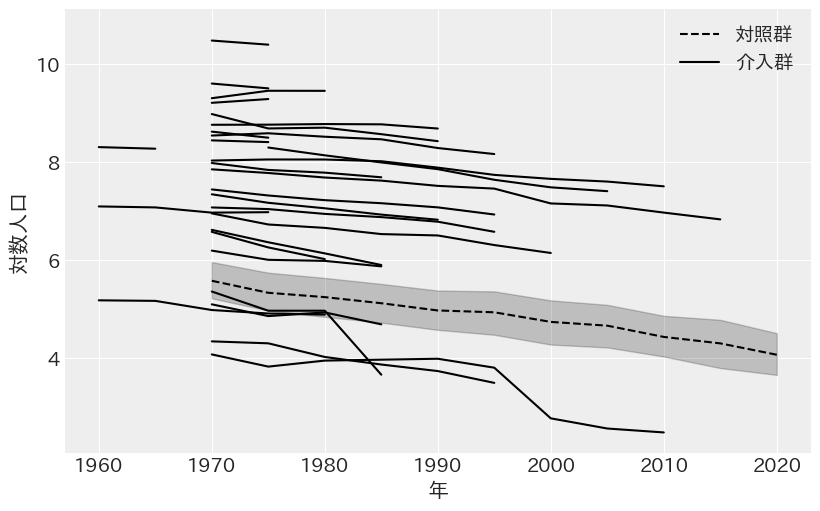
\includegraphics{../figures//pre_trend.png}
\caption{介入前トレンド}
\end{figure}

注: 人口データを元に筆者作成

\hypertarget{ux53cdux5b9fux4eeeux60f3ux306bux3088ux308bux4ecbux5165ux5f8cux306eux30c8ux30ecux30f3ux30c9ux691cux8a3c}{%
\subsubsection{\texorpdfstring{\(2.2.2\)
反実仮想による介入後のトレンド検証}{2.2.2 反実仮想による介入後のトレンド検証}}\label{ux53cdux5b9fux4eeeux60f3ux306bux3088ux308bux4ecbux5165ux5f8cux306eux30c8ux30ecux30f3ux30c9ux691cux8a3c}}

より厳密な検証として,介入群の介入前のデータのみを用いて,もし介入がなかった場合の反実仮想的なトレンドを予測し,対照群と比較することで平行トレンドの仮定を検証する.予測モデルには,島効果と年効果のみを考慮した以下の
Two-way Fixed Effects モデルを採用した.

\[
\begin{aligned}
\log{Y_{it}} &\sim \text{Student-t} (\nu, \mu_{it}, \sigma^2) \\
\nu &\sim \text{Gamma}(2, 0.1) \\
\mu_{it} &= \alpha_i + \lambda_t \\
\alpha_i &\sim \text{Normal}(\mu_{\alpha}, \sigma_{\alpha}^2) \\
\lambda_t &\sim \text{Normal}(\mu_{\lambda}, \sigma_{\lambda}^2) \\
\sigma &\sim \text{Cauchy}^+(1) \\
\end{aligned}
\]

添字 \(i\) は島,\(t\) は年を表す.被説明変数 \(\log{Y_{it}}\)
は対数人口であり,\(2.4\) 節にて述べるが,外れ値への対処のため 自由度
\(\nu\),平均 \(\mu\),分散 \(\sigma^2\) の \(t\)
分布に従うと仮定している.\(\alpha_i\) は島効果,\(\lambda_t\)
は年効果である.各事前分布は \(2.3\) 節にて説明する.

下図は介入後のトレンドを予測により補完した対数人口の推移を示している.

\begin{figure}
\centering
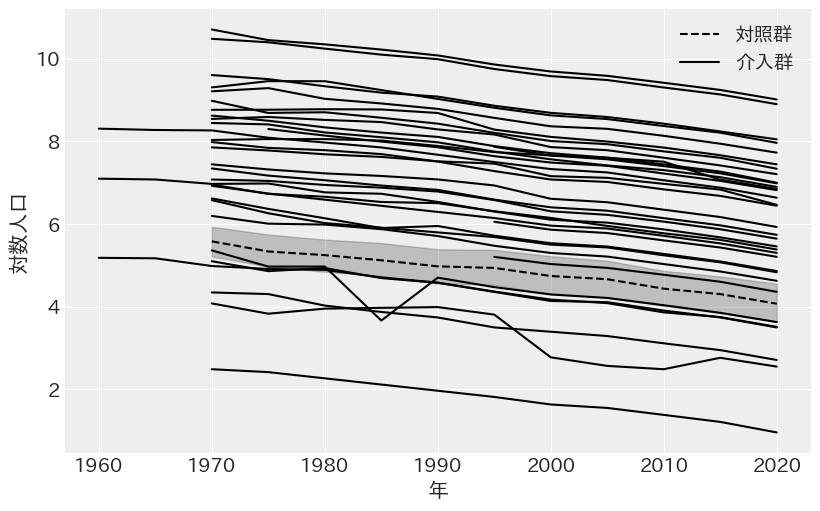
\includegraphics{../figures/post_trend.png}
\caption{介入後トレンド}
\end{figure}

注: 人口データを元に筆者作成

予測された介入群の反実仮想トレンドは,対照群の実際のトレンドと高い類似性を示している.より詳細な評価のため,\(95\%\)
信用区間を含む一部の予測結果を以下に示す.

\begin{figure}
\centering
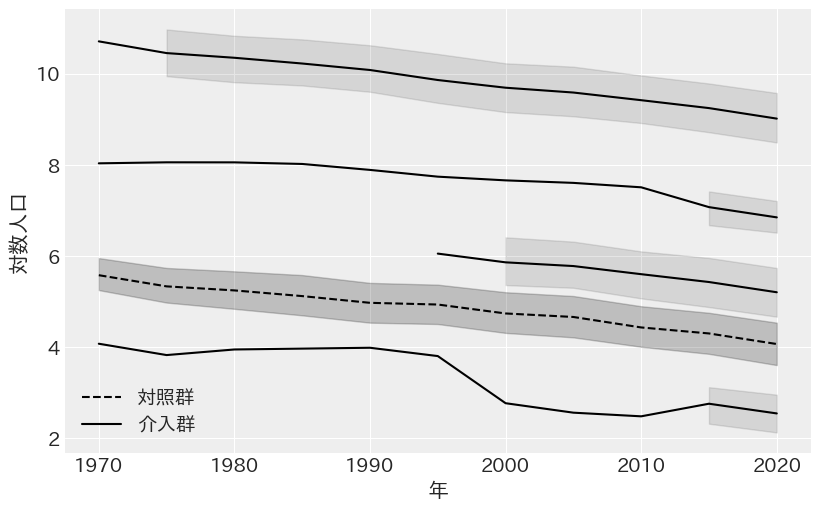
\includegraphics{../figures/post_trend_sample.png}
\caption{介入後トレンド抜粋}
\end{figure}

注: 人口データ及び予測値を元に筆者作成

ここからも介入群のトレンドは対照群のトレンドと類似していたことが示唆される.これらの分析結果から,本研究における平行トレンドの仮定は十分な妥当性を持つと判断できる.

本検証では \(2\) つの留意点がある.第 \(1\)
に対数変換前の実数人口においては平行トレンドの性質が必ずしも保持されない可能性がある.第
\(2\)
に,自己相関や単位根などの基本的な時系列特性を考慮していないため,より厳密な時系列分析を用いた追加検証の余地が残されている.ただし,これらの制約は本稿の主要な結論を大きく損なうものではないと考えられる.

\hypertarget{ux30e2ux30c7ux30eb}{%
\subsection{\texorpdfstring{\(2.3\)
モデル}{2.3 モデル}}\label{ux30e2ux30c7ux30eb}}

本稿では,離島架橋の介入効果を推定するために,以下の \(3\)
つのモデルを提案する.

\hypertarget{two-way-fixed-effects}{%
\subsubsection{\texorpdfstring{\(2.3.1\) Two-way Fixed
Effects}{2.3.1 Two-way Fixed Effects}}\label{two-way-fixed-effects}}

まずはじめのモデルとしては Two-way Fixed Effects (TWFE) を用いる.

\[
\begin{aligned}
\log{Y_{it}} &\sim \text{Student-t} (\nu, \mu_{it}, \sigma^2) \\
\nu &\sim \text{Gamma}(2, 0.1) \\
\mu_{it} &= \alpha_i + \lambda_t + \beta \cdot W_{it}\\
\alpha_i &\sim \text{Normal}(\mu_{\alpha}, \sigma_{\alpha}^2) \\
\lambda_t &\sim \text{Normal}(\mu_{\lambda}, \sigma_{\lambda}^2) \\
\beta &\sim \text{Normal}(0, 1) \\
\sigma &\sim \text{Cauchy}^+(1) \\
\end{aligned}
\]

被説明変数 \(\log{Y}_{it}\) は対数人口であり,自由度 \(\nu\) ,平均
\(\mu_{it}\) ,分散 \(\sigma_i^2\) の \(t\) 分布に従う.\(t\)
分布を使用することで外れ値に対してロバストな推定が可能になるが,詳細は自由度パラメータ
\(\nu\) とともに後ほど説明する.\(\mu_{it}\) の構造は島効果
\(\alpha_i\),年効果 \(\lambda_t\),介入効果 \(\beta\),介入変数
\(W_{it}\) によって構成される.島効果 \(\alpha_i\) は島 \(i\)
の固有の効果を示しており,ハイパーパラメータ \(\mu_{\alpha}\) と
\(\sigma_{\alpha}\)
によって平均と分散が決定される階層構造を仮定している.年効果
\(\lambda_t\) は年 \(t\)
の固有の効果を示しており,同様にハイパーパラメータ \(\mu_{\lambda}\) と
\(\sigma_{\lambda}\)
によって平均と分散が決定される階層構造を仮定している.介入効果 \(\beta\)
は介入の効果を示しており,事前分布として平均 \(0\),標準偏差 \(1\)
の正規分布を設定している.\(\sigma\)
は誤差分散を示しており,事前分布としてスケールパラメータ \(1\)
の半コーシー分布を設定している.以降では島効果と年効果のハイパーパラメータについて説明する.

下図は島別対数人口の平均値の分布である.

\begin{figure}
\centering
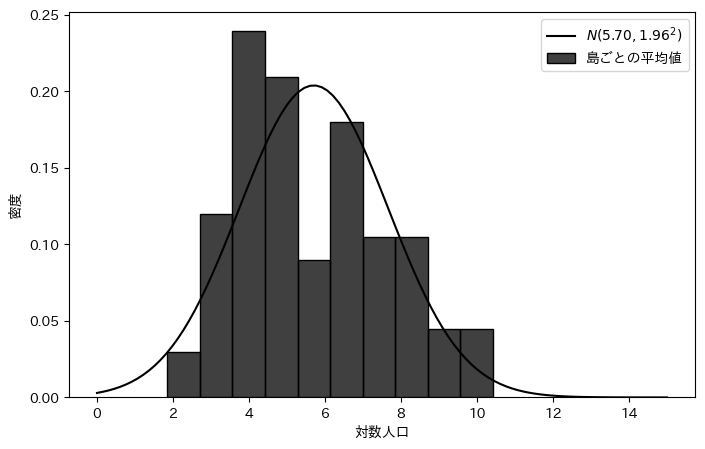
\includegraphics{../figures/define_models/mean_by_island.png}
\caption{島効果}
\end{figure}

注: 人口データを元に筆者作成

島ごとにグループ化した場合の対数人口の平均値の分布は,平均
\(5.78\),標準偏差 \(1.98\)
であり,島ごとの違いは以上のような正規分布から生成されていると仮定できる.したがって,島効果を個別に推定するのではなく,適切なハイパーパラメータを設定することで推定精度を向上させる.島効果の期待値
\(\mu_{\alpha}\) は \(6\),島効果の標準偏差 \(\sigma_{\alpha}\) は \(2\)
を中心に分布すると考え,それを事前分布として設定する.

\[
\begin{aligned}
\mu_{\alpha} &\sim \text{Normal}(6, 1) \\
\sigma_{\alpha} &\sim \text{Gamma}(3, 1) \\
\end{aligned}
\]

なお,これらの \(1\) というスケールは,\(\mu_{\alpha}\) がおよそ \(4\)
から \(8\),\(\sigma_{\alpha}\) が \(1.6\), \(8.2\)
になることを考えれば十分広いものだと考えられる.

年効果 \(\lambda_t\) は年 \(t\)
の固有の効果を示しており,ハイパーパラメータ \(\mu_{\lambda}\) と
\(\sigma_{\lambda}\) によって平均と分散が決定される.\(1960\)
年を基準にした対数人口の年平均は,平均 \(-0.968\),標準偏差は \(0.588\)
であった.

したがって,年効果の期待値 \(\mu_{\lambda}\) は \(-1\),年効果の標準偏差
\(\sigma_{\lambda}\) は \(0.6\)
を中心に分布すると考え,それを事前分布として以下のように設定する.

\[
\begin{aligned}
\mu_{\lambda} &\sim \text{Normal}(-1, 1) \\
\sigma_{\lambda} &\sim \text{Gamma}(2, 1) \\
\end{aligned}
\]

介入効果 \(\beta\) は介入の効果を示しており,事前分布として平均
\(0\),標準偏差 \(1\) の正規分布を設定する.これは橋の効果がおよそ
\(-2\) から \(2\).被説明変数が対数であることを考慮し,指数変換すると
\(-86\%\) から \(639\%\)
の範囲にあるという仮定であり,弱情報事前分布としては十分に広い範囲であると考えられる.

誤差分散 \(\sigma^2\) は事前分布としてスケールパラメータ \(1\)
の半コーシー分布を設定する.対数人口の標準偏差は \(2.02\)
であり,誤差項はモデルで説明できない変動であるため,誤差項の標準偏差がこれよりも大きい値を取ることはない.したがって,スケールパラメータ
\(1\) の半コーシー分布は十分に広い範囲をカバーしている.

\hypertarget{dynamic-twfe}{%
\subsubsection{\texorpdfstring{\(2.3.2\) Dynamic
TWFE}{2.3.2 Dynamic TWFE}}\label{dynamic-twfe}}

次に介入の動的な効果を測るため,Dynamic TWFE を用いる.

\[
\begin{aligned}
\log{Y_{it}} &\sim \text{Student-t} (\nu, \mu_{it}, \sigma^2) \\
\nu &\sim \text{Gamma}(2, 0.1) \\
\mu_{it} &= \alpha_i + \lambda_t + \sum_{\ell} \beta_{\ell} (\mathbb{1}\{t - E_i \in \ell\}) \\
\beta_{\ell} &\sim \text{Normal}(0, 1) \\
\sigma &\sim \text{Cauchy}^+(1) \\
\end{aligned}
\]

前述の TWFE との相違点は \(\mu_{it}\)
の構造にある.\(\mathbb{1}\{t - E_i \in \ell\}\) は,\(t\)
を観測年,\(E_i\) を島 \(i\) の介入年,\(\ell\)
を介入の経過年数として,介入の経過年数 \(\ell\)
における介入効果を示すダミー変数であり,\(\beta_{\ell}\)
は介入の経過年数 \(\ell\) における介入効果を示している.
このモデルは,介入効果が介入後に一定であるという TWFE
の仮定を緩和し,介入後の経過年数によって介入効果が変化することを考慮している.その他の事前分布は
TWFE と同様である.

\hypertarget{fully-saturated-twfe}{%
\subsubsection{2.3.3 Fully Saturated TWFE}\label{fully-saturated-twfe}}

Dynamic TWFE
では介入効果が介入後の経過年数によって変化することを考慮しているが,介入時期が異なる島間で介入効果が異なる場合にバイアスを持つ
(Sun \& Abraham 2021).したがって,介入効果の横断的な異質性を考慮した
Fully Saturated TWFE を用いる.

\[
\begin{aligned}
\log{Y_{it}} &\sim \text{Student-t} (\nu, \mu_{it}, \sigma^2) \\
\nu &\sim \text{Gamma}(2, 0.1) \\
\mu_{it} &= \alpha_i + \lambda_t + \sum_{e} \sum_{\ell} \beta_{e, \ell} (\mathbb{1}\{E_i \in e\} \cdot \{t - E_i \in \ell\}) \\
\beta_{e, \ell} &\sim \text{Normal}(0, 1) \\
\sigma &\sim \text{Cauchy}^+(1) \\
\end{aligned}
\]

\(\mathbb{1}\{E_i \in e\}\) は島 \(i\) の介入時期 \(e\)
を示すダミー変数であり,\(\beta_{e, \ell}\) は介入時期 \(e\)
の島における介入の経過年数 \(\ell\)
によって変動する介入効果を示している.

架橋には優先順位があり,介入時期が早い島と遅い島では効果が異なると考えるのが現実的だ.例えば効果が高いと見込まれたから早期から介入を受けた等の理由により異質性が生じる可能性が高い.このような状況では上述の
Dynamic TWFE ではバイアスが生じる.

介入を受けた時期に基づいて分類されたものをコホートとし,コホート別に介入効果の事後分布を推定することで
\(CATT_{e,\ell}\) (Cohort Average Treatment Effect on the Treated)
を得る.その後,各 CATT
を介入からの経過年数で分類し,経過年数別に平均を取る.その事後期待値を
\(\ell\) 時点の介入効果の期待値とし,事後標準偏差を \(\ell\)
時点の介入効果の標準偏差とする. 例えば,\(1990\) 年に出来た橋の \(5\)
年後の効果と \(2000\) 年に出来た橋の \(5\)
年後の効果を別々に推定した後,それらを平均することによって介入 \(5\)
年後の効果を推定する.

\hypertarget{ux5916ux308cux5024ux3078ux306eux5bfeux51e6ux3068ux9811ux5065ux306aux63a8ux5b9a}{%
\subsection{2.4
外れ値への対処と頑健な推定}\label{ux5916ux308cux5024ux3078ux306eux5bfeux51e6ux3068ux9811ux5065ux306aux63a8ux5b9a}}

本稿で使用するモデルでは,外れ値に対する頑健性を確保するた,被説明変数が
\(\text{Student-t}\)
分布に従うと仮定している.外れ値の影響を評価するため,まず診断的分析としてレバレッジの検討を行う.

レバレッジは観測値がデータ全体に与える影響の大きさを示す指標であり,
\(0\) から \(1\)
の値を取る.値が大きいほどその観測値がデータ全体に与える影響が大きく,潜在的な外れ値である可能性を示唆する.

Hoaglin \& Welsch(1978) に基づき,以下の手順でレバレッジを算出した.

まず,説明変数のデザイン行列 \(\mathbf{{X}}\) を用いてハット行列
\(\mathbf{H}\) を計算する.

\[
\mathbf{H} = \mathbf{X}(\mathbf{X}^{\top}\mathbf{X})^{-1}\mathbf{X}^{\top}
\]

次にハット行列の対角成分を取得し, \(i\) 番目の要素を \(L_i\)
として取得する.

\[
\text{L}_{i} = h_{ii}
\]

算出されたレバレッジの基本統計量と分布は以下の通りだ.

\begin{longtable}[]{@{}ccccc@{}}
\toprule
平均 & 標準偏差 & 最小 & 中央 & 最大\tabularnewline
\midrule
\endhead
\(0.115\) & \(0.032\) & \(0.093\) & \(0.106\) & \(0.388\)\tabularnewline
\bottomrule
\end{longtable}

\begin{figure}
\centering
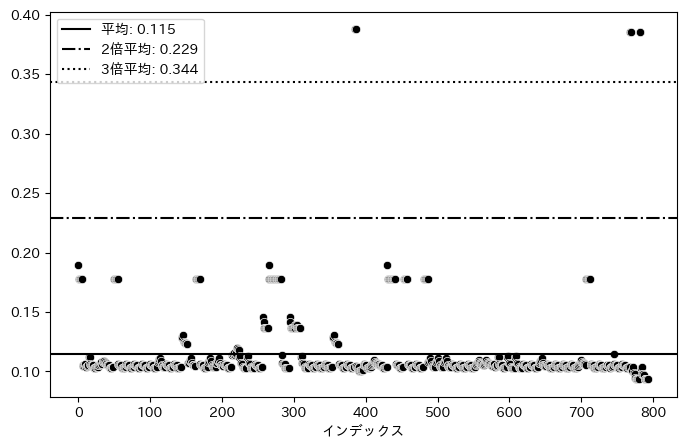
\includegraphics{../figures/define_models/leverage.png}
\caption{leverage}
\end{figure}

注: データを元に筆者作成

図において,横軸は観測番号,縦軸はレバレッジを示す.各水平線は下から順に平均レバレッジ,平均の
\(2\) 倍,\(3\) 倍の値を示している.一般的に平均レバレッジの \(2\) から
\(3\) 倍を超える観測値は外れ値として扱われる.本データセットでは平均の
\(3\) 倍を超える観測値が \(6\)
個検出されたため,これらを外れ値とみなす.このような外れ値が存在する場合,通常の正規分布を仮定したモデルでは推定結果が大きく歪む可能性がある.外れ値を除外する方法も考えられるが,重要な情報の損失を招く恐れがあるため,本稿では以下のように
\(\text{Student-t}\) 分布を用いたロバスト推定を採用する.

\[
\begin{aligned}
\log{Y_{it}} &\sim \text{Student-t} (\nu, \mu_{it}, \sigma_i^2) \\
\nu &\sim \text{Gamma}(2, 0.1) \\
\end{aligned}
\]

\(\text{Student-t}\) 分布は,自由度 \(\nu\)
が無限大に近づくと正規分布に収束する一方,自由度が小さい場合には正規分布よりも裾の重い分布となる.この特性により,外れ値が推定結果に与える影響を自然に抑制することが可能となる.自由度パラメータ
\(\nu\) の事前分布には,Juárez and Steel (2010) に従い
\(\text{Gamma}(2, 0.1)\)
を採用した.この設定により,データに応じて適切な自由度が推定され,モデルの柔軟性が確保される.

\hypertarget{ux5e73ux6ed1ux5316}{%
\subsection{2.5 平滑化}\label{ux5e73ux6ed1ux5316}}

Dynamic TWFE 及び Fully Saturated TWFE
では,動的な介入効果を計測する.推定結果については \(3.2\) 節および
\(3.3\)
節で述べるが,今回のデータセットでは介入効果の推定値が年ごとに大きく変動し,推定値の不安定性及び解釈の困難性が生じる可能性があり,この問題を解決するため,介入効果の推定値を以下の状態空間モデルを用いて平滑化する.

\[
\begin{aligned}
\delta_{\ell} &= \delta_{\ell-1} + \zeta_{\ell}, \quad &\zeta_{\ell} \sim \text{Normal}(0, \sigma_{\zeta}^2)\\
\mu_{\ell} &= \mu_{\ell-1} + \delta_{\ell-1} + w_{\ell}, \quad &w_{\ell} \sim \text{Normal}(0, \sigma_{w}^2)\\
\beta_{\ell} &= \mu_{\ell} + v_{\ell}, \quad &v_{\ell} \sim \text{Normal}(0, \sigma_{v}^2)\\
\end{aligned}
\]

\(\ell\) は経過年数であり,\(\delta_{\ell}\) は \(\ell\)
時点のトレンド,\(\mu_{\ell}\) は \(\ell\)
時点のレベル,\(\beta_{\ell}\) は \(\ell\)
時点の推定した介入効果の事後期待値を示している.\(\zeta_{\ell}\),\(w_{\ell}\),\(v_{\ell}\)
はそれぞれの誤差項であり,誤差項の分散の事前分布はスケールパラメータ
\(1\) の半コーシー分布とした.レベル \(\mu_{\ell}\) がトレンド
\(\delta_{\ell}\) や状態誤差 \(w_{\ell}\) によって変動し,その
\(\mu_{\ell}\) と観測誤差 \(v_{\ell}\) によって介入効果 \(\beta_{\ell}\)
が生成されるというモデルである. そのように推定したレベル \(\mu_{\ell}\)
を平滑化した介入効果の事後期待値として解釈する.なお,平滑化しない推定量の
\(95\%\) 信用区間の評価には観測誤差 \(\zeta_{\ell}\) は使用せず,Dynamic
TWFE や Fully Saturated TWFE
によって推定された信用区間を用いて評価する.

\hypertarget{ux5206ux6790ux7d50ux679c}{%
\section{3. 分析結果}\label{ux5206ux6790ux7d50ux679c}}

\hypertarget{two-way-fixed-effect}{%
\subsection{3.1 Two-way fixed effect}\label{two-way-fixed-effect}}

下の表は介入後の効果を一定と仮定する Two-way Fixed Effects
モデルの推定結果である.

\begin{longtable}[]{@{}cccccc@{}}
\toprule
params & EAP & post.sd & 95\%下限 & 95\%上限 &
\(\hat{R}\)\tabularnewline
\midrule
\endhead
\(\beta\) & \(0.208\) & \(0.031\) & \(0.151\) & \(0.266\) &
\(1.0\)\tabularnewline
\(\mu_{\text{island}}\) & \(6.342\) & \(0.249\) & \(5.858\) & \(6.794\)
& \(1.0\)\tabularnewline
\(\sigma_{\text{island}}\) & \(1.994\) & \(0.161\) & \(1.702\) &
\(2.307\) & \(1.0\)\tabularnewline
\(\mu_{\text{year}}\) & \(-0.659\) & \(0.202\) & \(-1.048\) & \(-0.285\)
& \(1.0\)\tabularnewline
\(\sigma_{\text{year}}\) & \(0.577\) & \(0.146\) & \(0.345\) & \(0.846\)
& \(1.0\)\tabularnewline
\(\sigma\) & \(0.143\) & \(0.009\) & \(0.126\) & \(0.160\) &
\(1.0\)\tabularnewline
\(\nu\) & \(2.221\) & \(0.271\) & \(1.731\) & \(2.728\) &
\(1.0\)\tabularnewline
\bottomrule
\end{longtable}

注: \(\beta\) は介入効果を示すパラメータ.\(\mu_{\text{island}}\)
は島効果の期待値のハイパーパラメータ.\(\sigma_{\text{island}}\)
は島効果の分散のハイパーパラメータ.\(\mu_{\text{year}}\)
年効果の期待値のハイパーパラメータ.\(\sigma_{\text{year}}\)
は年効果の分散のハイパーパラメータ.\(\sigma\)
は誤差項の標準偏差.\(\nu\) は \(\text{Student-t}\)
分布の自由度パラメータ.EAP は事後期待値.post.sd
は事後標準偏差.95\%下限及び 95\%上限は信用区間.\(\hat{R}\)
はゲルマン・ルービンの収束診断であり 1.1 以下で収束したと判断する.

介入効果を示すパラメータである \(\beta\) は \(0.208\)
と推定された.\(95\%\) 信用区間は \(0\)
を含まず,介入効果が正,つまり介入後には介入前より人口が増加する確率は
\(100\%\)
と推定された.被説明変数は対数値であるため指数変換により評価すると架橋後の人口は平均
\(23.18\%\) 増加する.

\hypertarget{dynamic-twfe-1}{%
\subsection{3.2 Dynamic TWFE}\label{dynamic-twfe-1}}

下の表は介入の効果を時間変化させる Dynamic TWFE モデルの推定結果である.

\begin{longtable}[]{@{}cccccc@{}}
\toprule
param & EAP & post.sd & 95\% 下側 & 95\% 上側 &
\(\hat{R}\)\tabularnewline
\midrule
\endhead
\(\mu_{\text{island}}\) & \(6.489\) & \(0.258\) & \(5.993\) & \(7.006\)
& \(1.0\)\tabularnewline
\(\sigma_{\text{island}}\) & \(1.966\) & \(0.163\) & \(1.646\) &
\(2.284\) & \(1.0\)\tabularnewline
\(\mu_{\text{year}}\) & \(-0.758\) & \(0.225\) & \(-1.196\) & \(-0.304\)
& \(1.0\)\tabularnewline
\(\sigma_{\text{year}}\) & \(0.643\) & \(0.161\) & \(0.380\) & \(0.951\)
& \(1.0\)\tabularnewline
\(\sigma\) & \(0.119\) & \(0.010\) & \(0.101\) & \(0.138\) &
\(1.0\)\tabularnewline
\(\nu\) & \(1.881\) & \(0.231\) & \(1.452\) & \(2.329\) &
\(1.0\)\tabularnewline
\bottomrule
\end{longtable}

注: \(\mu_{\text{island}}\)
は島効果の期待値のハイパーパラメータ.\(\sigma_{\text{island}}\)
は島効果の分散のハイパーパラメータ.\(\mu_{\text{year}}\)
年効果の期待値のハイパーパラメータ.\(\sigma_{\text{year}}\)
は年効果の分散のハイパーパラメータ.\(\sigma\)
は誤差項の標準偏差.\(\nu\) は \(\text{Student-t}\)
分布の自由度パラメータ.EAP は事後期待値.post.sd
は事後標準偏差.95\%下限及び 95\%上限は信用区間.\(\hat{R}\)
はゲルマン・ルービンの収束診断であり 1.1 以下で収束したと判断する.

島効果や年効果,誤差分散,自由度は TWFE
と同様の結果が得られた.介入効果の時間変化を示すパラメータは下図で示す.

\begin{figure}
\centering
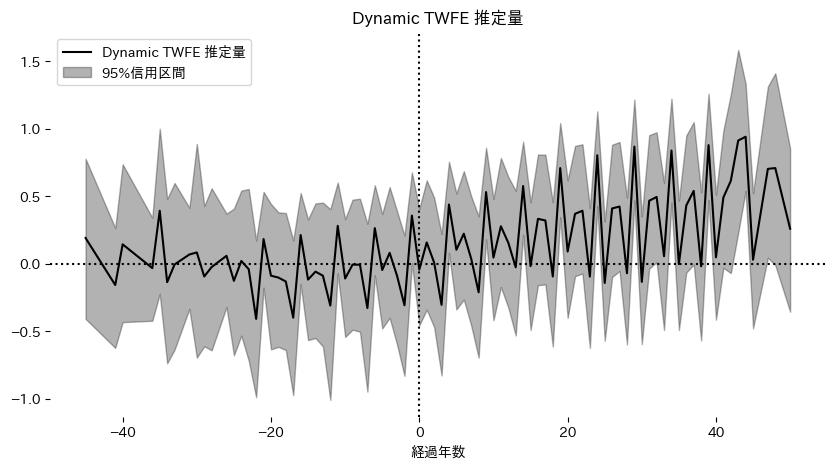
\includegraphics{../figures/dynamic_twfe/ATT.png}
\caption{時変介入効果}
\end{figure}

注: 推定結果を元に筆者作成

介入前 \(46\) 年から介入後 \(50\)
年まで推定した介入効果の時間変化を示す.介入前は \(0\)
付近で変動し,介入後は効果が上昇することがわかる.

下の表は介入前から介入後までの各経過年数期間における事後期待値とパラメータが正である確率を示している.介入前の全期間における期待値は
\(-8.095\%\) であり,パラメータが正である確率は \(39.278\%\)
である.すなわち,介入前は人口が約 \(8\%\)
少ない.一方,介入後の全期間における期待値は \(29.605\%\)
であり,パラメータが正である確率は \(73.440\%\)
である.すなわち,介入後は人口が約 \(30\%\)
増加するといえる.また,介入前で最も人口減少を経験しているのは
\(-30 \sim -21\) 年の期間であり,EAP は \(13\%\)
であり,この期間が特に人口が減っているが,他の期間はあまり変わらない.一方,介入後は徐々に期待値が増加しており,最も人口増加を経験しているのは
\(31 \sim 40\) 年でピークを迎え,約 \(54\%\) 増加している.

\begin{longtable}[]{@{}ccccccc@{}}
\toprule
介入前 & EAP & 正の確率 & & 介入後 & EAP & 正の確率\tabularnewline
\midrule
\endhead
全期間 & \(-8.095\%\) & \(39.278\%\) & & 全期間 & \(29.605\%\) &
\(73.440\%\)\tabularnewline
\(-10 \sim -2\) & \(-6.519\%\) & \(43.492\%\) & & \(0 \sim 10\) &
\(14.038\%\) & \(66.862\%\)\tabularnewline
\(-20 \sim -11\) & \(-4.438\%\) & \(41.055\%\) & & \(11 \sim 20\) &
\(28.899\%\) & \(75.097\%\)\tabularnewline
\(-30 \sim -21\) & \(-13.388\%\) & \(31.710\%\) & & \(21 \sim 30\) &
\(25.412\%\) & \(68.020\%\)\tabularnewline
\(-46 \sim -31\) & \(-8.829\%\) & \(39.828\%\) & & \(31 \sim 40\) &
\(53.903\%\) & \(83.784\%\)\tabularnewline
- & - & - & & \(41 \sim 50\) & \(30.787\%\) &
\(74.255\%\)\tabularnewline
\bottomrule
\end{longtable}

注: EAP は指数変換による事後期待値.

また,一見すると短期的な変動が激しいように見えるが,本来はこのような激しさは持たず,個別の橋の効果が強く出てしまっているだけだと考えられる.なぜなら,国勢調査では
\(5\) 年毎でしかデータが得られず,介入年が \(1\)
年異なると各経過年数毎ではサンプルサイズが小さくなってしまうといった事情があるからだ.たとえば,\(1990\)
年に架かった橋と \(1991\) 年に架かった橋があるとき,\(1995\)
年のデータは前者は \(5\) 年目の効果,後者は \(4\)
年目の効果のために使用される.そのため経過年数 \(-5\) 年や,経過年数
\(0\) 年,経過年数 \(10\)
年といったダミー変数によってそれぞれの効果を推定しているが,これらの変数の中で
\(1\) をとる割合は平均的に \(0.5\%\)
程度と小さくなる.したがって両者の島の介入効果に異質性がある場合,個別の橋の効果が強く出てしまうだろう.そこで,得られた推定値に対して状態空間モデルを用いて平滑化を行なった.

誤差項の分散は以下のように推定された.トレンドの誤差項の分散
\(\sigma_{\zeta}\) とレベルの誤差項の分散 \(\sigma_{w}\)
の期待値はそれぞれ \(0.002\) と \(0.018\)
であるが,それに比べて介入効果の誤差項の分散 \(\sigma_{v}\) は \(0.229\)
と大きい.

\begin{longtable}[]{@{}cccccc@{}}
\toprule
param & EAP & post.sd & 95\% 下側 & 95\% 上側 &
\(\hat{R}\)\tabularnewline
\midrule
\endhead
\(\sigma_{\zeta}\) & \(0.002\) & \(0.002\) & \(0\) & \(0.006\) &
\(1.0\)\tabularnewline
\(\sigma_{w}\) & \(0.018\) & \(0.013\) & \(0\) & \(0.043\) &
\(1.0\)\tabularnewline
\(\sigma_{v}\) & \(0.229\) & \(0.018\) & \(0.196\) & \(0.265\) &
\(1.0\)\tabularnewline
\bottomrule
\end{longtable}

注: \(\sigma_{\zeta}\) はトレンドの誤差項の分散.\(\sigma_{w}\)
はレベルの誤差項の分散.\(\sigma_{v}\) は介入効果の誤差項の分散.EAP
は事後期待値.post.sd は事後標準偏差.95\%下限及び
95\%上限は信用区間.\(\hat{R}\) はゲルマン・ルービンの収束診断であり 1.1
以下で収束したと判断する.

以下は平滑化された Dynamic TWFE 推定量を示している.

\begin{figure}
\centering
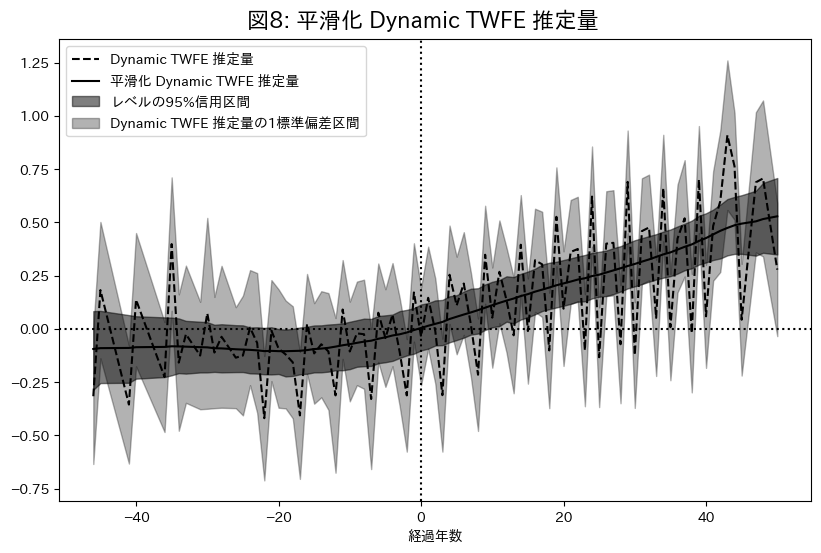
\includegraphics{../figures/dynamic_twfe/smoothed_ATT.png}
\caption{平滑化介入効果}
\end{figure}

注: 推定結果を元に筆者作成

破線は平滑化をしていない介入効果の期待値であり,実線は平滑化した期待値,濃い灰色の帯はレベル
\(\mu_{\ell}\) の\(95\%\) 信用区間,薄い灰色の帯は Dynamic TWFE 推定量の
\(95\%\)
信用区間である.平滑化を行うことで介入効果の時間変化が滑らかになり,解釈性が向上した.平滑化期待値は,介入前
\(-40\) 年はほぼ \(0\) であり,\(-20\)
年に向けて低下しているが,その後は方向を変えて徐々に上昇し,介入の 5
年前には期待値が \(0.003\) と正に転換した.介入 \(8\) 年目にはレベル
\(\mu_{\ell}\) の \(95\%\) 信用区間が \(0\) を含まなくなり,期待値は
\(0.13\) に達している.その後の期待値は負になることなく上昇し,\(50\)
年目の期待値は \(0.55\) となった.一方で介入効果の信用区間は最後まで
\(0\)
を含んでいるが,これは,介入効果の出やすい島と出づらい島といった横断的な異質性が大きいためだと考えられる.しかし,負の割合は経過年数が進むにつれて減少しており,少なくとも人口減少を抑制する効果があることが示されている.

ここから言えることは,離島架橋は平均的に人口減少を改善させる可能性が高く,全てのケースにおいて人口増加をもたらすわけではないかもしれないが,少なくとも人口減少を抑制する効果があることが示されている.

\hypertarget{fully-saturated-twfe-1}{%
\subsection{3.3 Fully Saturated TWFE}\label{fully-saturated-twfe-1}}

時系列的な異質性に加え,横断的な異質性を考慮した Fully Saturated TWFE
の推定結果は以下の通りである.

\begin{longtable}[]{@{}cccccc@{}}
\toprule
param & EAP & post.sd & 95\% 下側 & 95\% 上側 &
\(\hat{R}\)\tabularnewline
\midrule
\endhead
\(\mu_{\text{island}}\) & \(5.930\) & \(0.358\) & \(4.968\) & \(6.890\)
& \(1.0\)\tabularnewline
\(\sigma_{\text{island}}\) & \(1.975\) & \(0.159\) & \(1.674\) &
\(2.311\) & \(1.0\)\tabularnewline
\(\mu_{\text{year}}\) & \(-0.193\) & \(0.337\) & \(-1.112\) & \(0.762\)
& \(1.0\)\tabularnewline
\(\sigma_{\text{year}}\) & \(0.626\) & \(0.157\) & \(0.372\) & \(0.946\)
& \(1.0\)\tabularnewline
\(\sigma\) & \(0.137\) & \(0.011\) & \(0.116\) & \(0.160\) &
\(1.0\)\tabularnewline
\(\nu\) & \(2.446\) & \(0.365\) & \(1.766\) & \(3.181\) &
\(1.0\)\tabularnewline
\bottomrule
\end{longtable}

注: \(\mu_{\text{island}}\)
は島効果の期待値のハイパーパラメータ.\(\sigma_{\text{island}}\)
は島効果の分散のハイパーパラメータ.\(\mu_{\text{year}}\)
年効果の期待値のハイパーパラメータ.\(\sigma_{\text{year}}\)
は年効果の分散のハイパーパラメータ.\(\sigma\)
は誤差項の標準偏差.\(\nu\) は \(\text{Student-t}\)
分布の自由度パラメータ.EAP は事後期待値.post.sd
は事後標準偏差.95\%下限及び 95\%上限は信用区間.\(\hat{R}\)
はゲルマン・ルービンの収束診断であり 1.1 以下で収束したと判断する.

島効果や年効果,誤差分散,自由度は TWFE,Dynamic TWFE
と同様の結果が得られた.\(\beta_{e, \ell}\)
は介入年別及び経過年数別に合計 \(250\)
個の介入効果を推定している.その後同じ経過年数を持つパラメータの事後分布を平均し,経過年数別の介入効果を推定した.その結果が以下のグラフである.

\begin{figure}
\centering
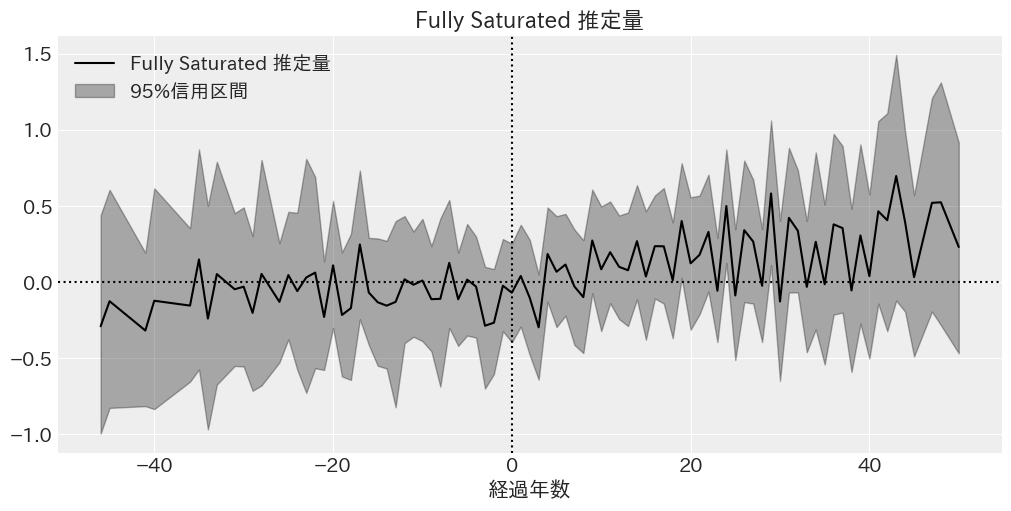
\includegraphics{../figures/fully_saturated_twfe/ATT.png}
\caption{Fully saturated TWFE 推定量}
\end{figure}

注: 推定結果を元に筆者作成

横軸は介入年を \(0\)
とした経過年数,縦軸は介入効果を示している.介入前は \(0\)
の周辺もしくはやや \(0\)
以下に偏った形で分布しているが,介入後は正の方向に向かっていることがわかる.

事後分布のサンプルからそれぞれの期間において \(0\)
を上回る確率を計算した結果を下の表にまとめた.介入前の全期間における期待値は
\(-7%
\) であり,パラメータが正である確率は \(38.574\%\)
である.一方,介入後の全期間における期待値は \(20.126\%\)
であり,パラメータが正である確率は \(70.884\%\)
である.すなわち,介入後は人口が約 \(20\%\) 増加する.また,Dynamic TWFE
による推定では \(-30 \sim -21\)
年の期間が最も人口減少を経験していたが,Fully Saturated TWFE
による推定では \(-46 \sim -31\)
年の期間が最も人口減少を経験している.一方で,介入後は Dynamic TWFE
よりも介入後の期待値は小さく推定され,最初の 10 年間は約 \(1.5\%\)
の効果しかなく,正である確率も \(50\%\)
である.その後は効果が上昇し,最後の \(10\) 年間である \(41 \sim 50\)
年の期間が最も人口増加を経験しており,ピークは \(50\%\) を超えている.

\begin{longtable}[]{@{}ccccccc@{}}
\toprule
介入前 & EAP & 正の確率 & & 介入後 & EAP & 正の確率\tabularnewline
\midrule
\endhead
全期間 & \(-7.332\%\) & \(38.574\%\) & & 全期間 & \(20.126\%\) &
\(70.884\%\)\tabularnewline
\(-10 \sim -2\) & \(-8.231\%\) & \(35.713\%\) & & \(0 \sim 10\) &
\(1.488\%\) & \(53.516\%\)\tabularnewline
\(-20 \sim -11\) & \(-5.108\%\) & \(41.383\%\) & & \(11 \sim 20\) &
\(18.282\%\) & \(77.599\%\)\tabularnewline
\(-30 \sim -21\) & \(-5.051\%\) & \(40.864\%\) & & \(21 \sim 30\) &
\(20.837\%\) & \(70.420\%\)\tabularnewline
\(-46 \sim -31\) & \(-11.555\%\) & \(35.517\%\) & & \(31 \sim 40\) &
\(22.058\%\) & \(72.449\%\)\tabularnewline
- & - & - & & \(41 \sim 50\) & \(50.342\%\) &
\(84.995\%\)\tabularnewline
\bottomrule
\end{longtable}

注: EAP は指数変換による事後期待値.

Dynamic TWFE と同様に,同様の状態空間モデルを用いて平滑化を行なった.

以下の表は状態空間モデルで推定した \(3\)
つの誤差項の分散の推定結果である.トレンドの誤差項の分散
\(\sigma_{\zeta}\) とレベルの誤差項の分散 \(\sigma_{w}\)
の期待値はそれぞれ \(0.002\) と \(0.016\) であり,Dynamic TWFE
と比べても大きな変化はない.しかし,介入効果の誤差項の分散
\(\sigma_{v}\) は \(0.170\) と Dynamic TWFE よりも小さく推定された.

\begin{longtable}[]{@{}cccccc@{}}
\toprule
params & EAP & post.sd & 95\%下限 & 95\%上限 &
\(\hat{R}\)\tabularnewline
\midrule
\endhead
\(\sigma_{\zeta}\) & \(0.002\) & \(0.002\) & \(0\) & \(0.006\) &
\(1.0\)\tabularnewline
\(\sigma_{w}\) & \(0.016\) & \(0.012\) & \(0\) & \(0.040\) &
\(1.0\)\tabularnewline
\(\sigma_{v}\) & \(0.170\) & \(0.014\) & \(0.144\) & \(0.197\) &
\(1.0\)\tabularnewline
\bottomrule
\end{longtable}

注: \(\sigma_{\zeta}\) はトレンドの誤差項の分散.\(\sigma_{w}\)
はレベルの誤差項の分散.\(\sigma_{v}\) は介入効果の誤差項の分散.EAP
は事後期待値.post.sd は事後標準偏差.95\%下限及び
95\%上限は信用区間.\(\hat{R}\) はゲルマン・ルービンの収束診断であり 1.1
以下で収束したと判断する.

下図は平滑化された Fully Saturated TWFE 推定量を示している.

\begin{figure}
\centering
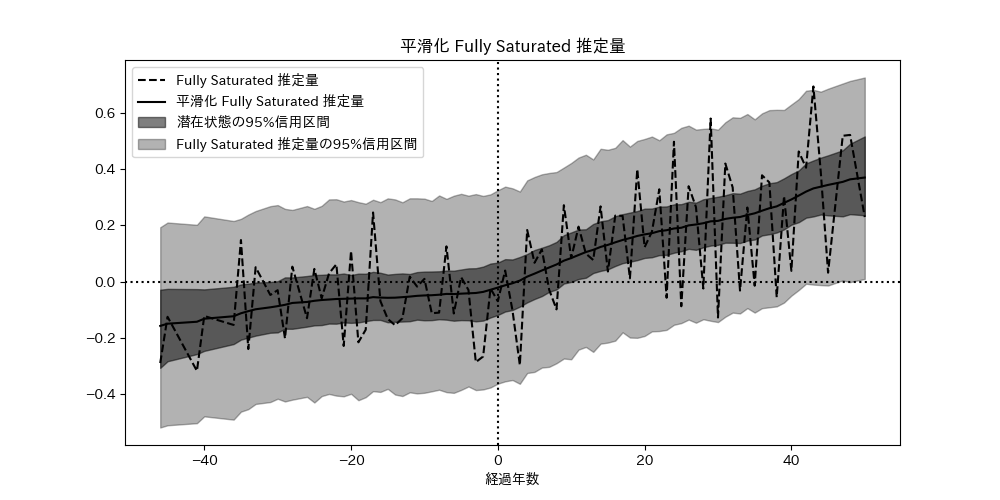
\includegraphics{../../docs/figures/fully_saturated_twfe/smoothed_ATT.png}
\caption{平滑化 Fully saturated TWFE 推定量}
\end{figure}

注: 推定結果を元に筆者作成

破線は平滑化をしていない介入効果の期待値であり,実線は平滑化した期待値,濃い灰色の帯はレベル
\(\mu_{\ell}\) の \(95\%\) 信用区間,薄い灰色の帯は Fully Saturated TWFE
推定量の \(95\%\)
信用区間である.平滑化を行うことで介入効果の時間変化が滑らかになり,解釈性が向上した.平滑化推定量は,介入前は常に負の値を取っており,
\(-30\) 年から \(0\)
は横ばいで推移している.介入年から傾きが変わって上昇し,人口に正の影響を与えていることがわかる.

この節の最後に Fully saturated TWFE と Dynamic TWFE
の平滑化推定量を比較する.

\begin{figure}
\centering
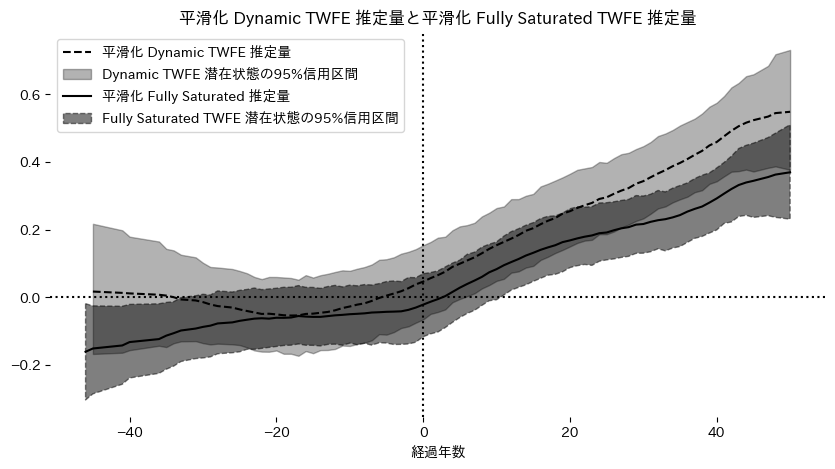
\includegraphics{../../docs//figures//fully_saturated_twfe//fs_vs_dynamic.png}
\caption{FullySaturated VS Dynamic}
\end{figure}

注: 推定結果を元に筆者作成

実線は Fully saturated TWFE の平滑化推定量,破線は Dynamic TWFE
の平滑化推定量である.Dynamic TWFE
は効果が大きく推定されている傾向にある.\(-40\)
年の期待値はわずかに正である事に加え,\(‐18\)
年を最小値としてその後は介入効果が上昇している.一方で Fully saturated
TWFE は基本的に Dynamic TWFE
よりも小さく推定されている.介入前は負の値を取っており,介入効果の上昇は
\(0\) または数年前から始まっている.Dynamic TWFE
は介入前の効果を高く推定するバイアスがあり\footnote{DOORS 編集部
  \((2024)\) でも同様に介入前の効果を高く推定する傾向があった.} ,Fully
saturated の方が現実的な推定値を示していると言える.

\hypertarget{ux8003ux5bdf}{%
\subsection{4. 考察}\label{ux8003ux5bdf}}

この章では,Fully Saturated TWFE で得られた \(CATT_{e, \ell}\) 計 \(23\)
個の中から抜粋し,島の実際の人口変化率との比較をすることで橋の効果を考察する.

下図は広島県尾道市生口島に \(1991\)
年に開通した生口橋の効果を示している.このサンプルは最も架橋によって人口が増加したと推定されたサンプルであり,係数は介入前
\(-1\) 年では \(-33.50\%\) \footnote{指数変換により算出.以後断りがない限り指数変換による値を示す.}
であったのに比べて,介入 \(4\) 年後には \(56.99\%\)
を示した.その後の人口変化率は介入前と同じような傾きで減少しているため,介入効果は一時的なものと思われるかもしれないが,係数は上昇を続けている.

\begin{figure}
\centering
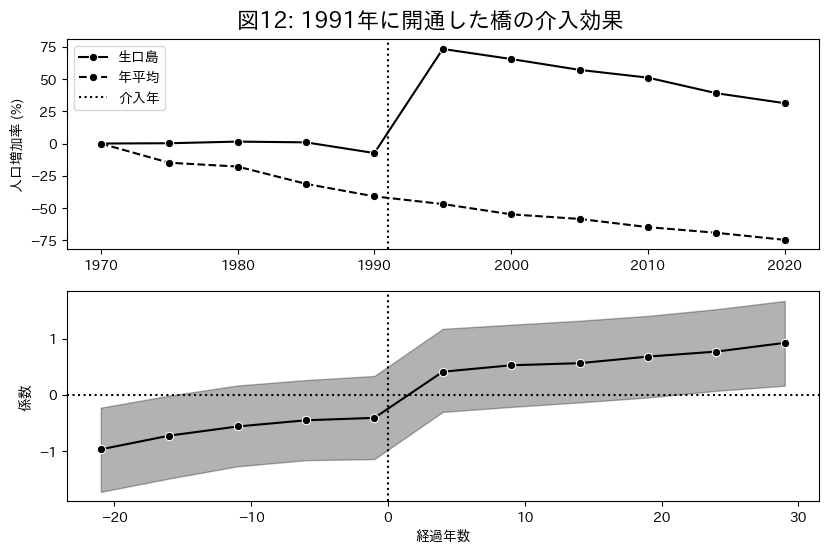
\includegraphics{../figures/fully_saturated_twfe/1991.png}
\caption{介入 1991 年}
\end{figure}

注:
人口データ及び推定結果を元に筆者作成.上段の実線は人口の最初の観測値を基準にした変化率.上段の破線は研究対象の全島人口の年平均変化率.下段の実線は
Fully Saturated TWFE による介入効果 \(CATT_{1991, \ell}\)
の推定値.下段の帯は \(95\%\) 信用区間.両パネルの縦の点線は介入年.

下図は広島県江田島市沖野島に \(1972\)
年に開通した早瀬大橋の効果を示している.こちらは一時的なストロー効果を経験したが,その後長年かけて正の効果が出た例である.介入後の
\(3\) 年間で人口が急激に減少し約 \(-50\%\) となった.その後は \(23\)
年後までデータが得られていないため,その間の推移は不明であるが,もし同様の傾向が続いているとすれば,架橋によってストロー効果が引き起こされたと考えるかもしれない.しかし,長年かけて年平均の減少率に追いつき,架橋から
\(28\) 年目には人口増加率が年平均を上回った.介入から \(43\)
年後の係数は信用区間を考慮しても \(0\) を上回るようになり,期待値は
\(100.57\%\)
となった.ここまで効果が高いのは何か他に要因があるだろうが,架橋によって将来の人口減少が抑制されたと考えることもできる.

\begin{figure}
\centering
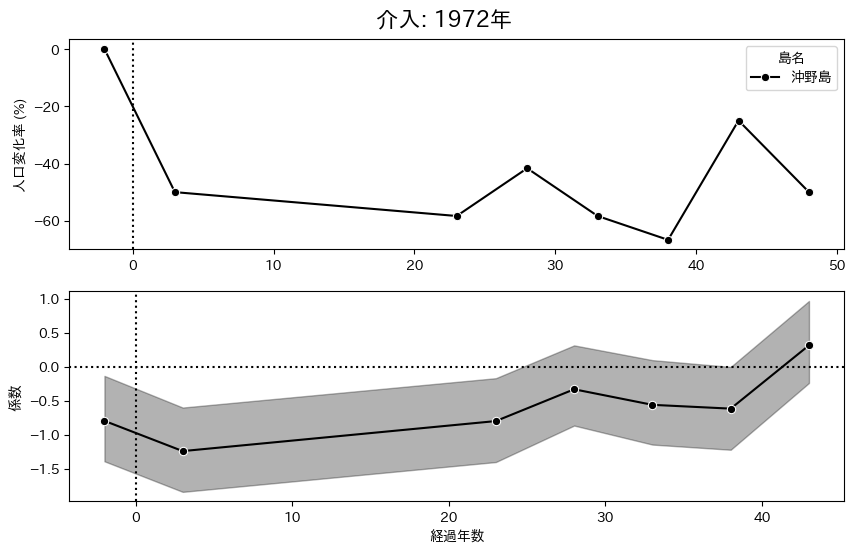
\includegraphics{../figures/fully_saturated_twfe/1972.png}
\caption{介入 1972 年}
\end{figure}

注:
人口データ及び推定結果を元に筆者作成.上段の実線は人口の最初の観測値を基準にした変化率.上段の破線は研究対象の全島人口の年平均変化率.下段の実線は
Fully Saturated TWFE による介入効果 \(CATT_{1972, \ell}\)
の推定値.下段の帯は \(95\%\) 信用区間.両パネルの縦の点線は介入年.

下図は高知県須崎市中ノ島に \(1982\)
年に架かった中ノ島大橋の効果を示している.上段の実績値を見ると架橋によって人口が増加しているように見える.しかし係数では介入前
\(-12\) 年で \(-46.15\%\) と最も小さな値を取るが,次の \(-7\) 年目では
\(-35.53\%\)
となりそこから係数が増加しており,介入前から効果が現れている.個別の橋の建設期間を調査するのは難しいが,明石海峡大橋を参考にすると着工から完成まで
\(12\) 年掛かる\footnote{鹿島建設の資料によると \(1986\)
  年着工.\(1998\) 年完成.}.それよりは短いと考えられるが,\(5\)
年以上の期間があると仮定すると,橋の建設開始がその島の経済の見通しを明るくしたために人口増加を引き起こしたと考えられる.

\begin{figure}
\centering
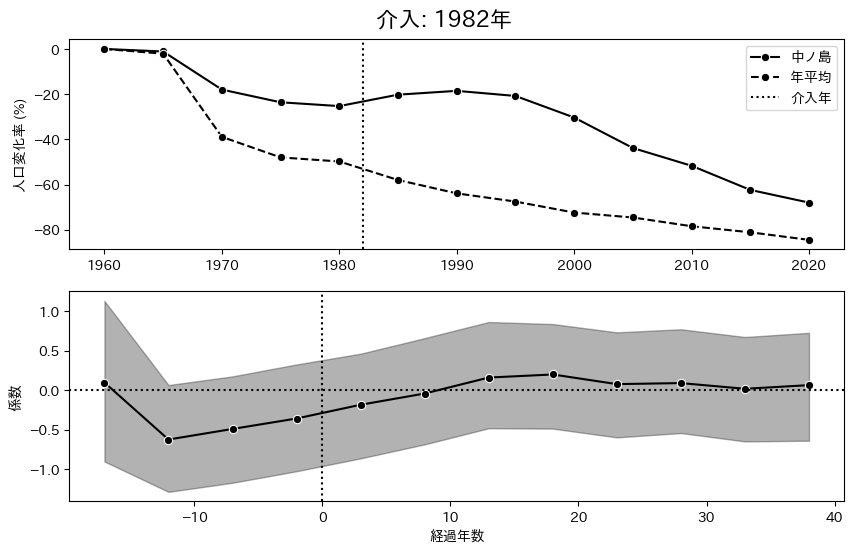
\includegraphics{../figures/fully_saturated_twfe/1982.png}
\caption{介入 1982 年}
\end{figure}

注:
人口データ及び推定結果を元に筆者作成.上段の実線は人口の最初の観測値を基準にした変化率.上段の破線は研究対象の全島人口の年平均変化率.下段の実線は
Fully Saturated TWFE による介入効果 \(CATT_{1982, \ell}\)
の推定値.下段の帯は \(95\%\) 信用区間.両パネルの縦の点線は介入年.

下図は広島県福山市田島に \(1989\)
年に開通した内海大橋の効果を示す.こちらは介入前 \(-19\) 年から \(‐9\)
年までは年平均と同様の動きをするが,介入前 \(-4\)
年から人口減少率が小さくなり,以降は年平均と徐々に差が開くようになる.こちらも開通年より先に効果が出ている例である.また,もし年平均を無視すれば架橋していても減少傾向には変わりないため,ストロー効果があると解釈される事があるかもしれない.しかし,年平均を考慮すれば明らかに架橋によって人口減少が抑制されており,係数を見ても右肩上がりであり,介入後
\(6\) 年の期待値を見ると区間は広いものの
\(11.63\%\).の効果があることがわかる.

\begin{figure}
\centering
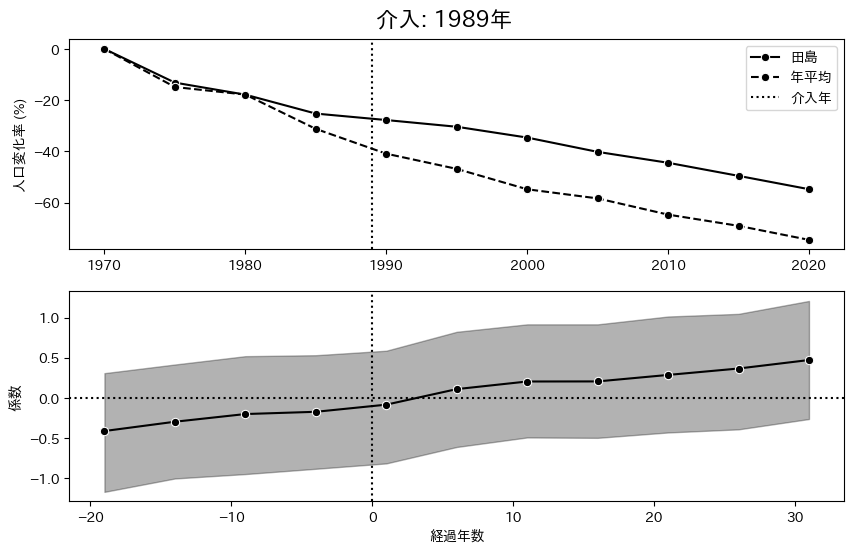
\includegraphics{../figures/fully_saturated_twfe/1989.png}
\caption{介入 1989 年}
\end{figure}

注:
人口データ及び推定結果を元に筆者作成.上段の実線は人口の最初の観測値を基準にした変化率.上段の破線は研究対象の全島人口の年平均変化率.下段の実線は
Fully Saturated TWFE による介入効果 \(CATT_{1989, \ell}\)
の推定値.下段の帯は \(95\%\) 信用区間.両パネルの縦の点線は介入年.

下図は広島県大崎上島町にある長島に \(1987\)
年に開通した長島大橋である.これは最も効果が悪い例であり,介入前 \(-7\)
から介入前 \(-2\)
年にかけて急激に人口が減った上,介入後の効果もずっと負である.\(1980\)
年時点では人口は \(144\) 人いたが,\(1985\) 年には \(39\)
人に減ってしまった.中國新聞 (1998) によると,\(1978\)
年に火力発電所の建設が決まり,島民が集団移転するという事情があった.しかし中國新聞には島民の声が掲載されており,橋ができたことで
1
時間半歩いて病院に通えるため住むには良いところだという意見があった.もし橋が無ければ人口流出が抑えられず,火力発電所の従業員のみが暮らす島になっている可能性はあるが,橋ができたことで残された島民の生活が改善されたと考えることもできる.

\begin{figure}
\centering
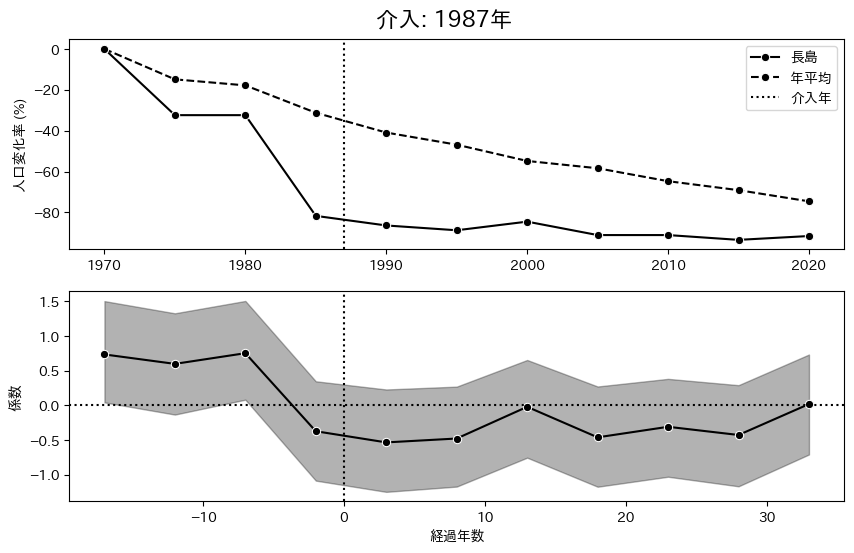
\includegraphics{../figures/fully_saturated_twfe/1987.png}
\caption{介入 1987 年}
\end{figure}

注:
人口データ及び推定結果を元に筆者作成.上段の実線は人口の最初の観測値を基準にした変化率.上段の破線は研究対象の全島人口の年平均変化率.下段の実線は
Fully Saturated TWFE による介入効果 \(CATT_{1987, \ell}\)
の推定値.下段の帯は \(95\%\) 信用区間.両パネルの縦の点線は介入年.

\hypertarget{ux307eux3068ux3081}{%
\subsection{5. まとめ}\label{ux307eux3068ux3081}}

本研究では,離島架橋の効果を因果推論の手法を用いて推定した.時系列的及び横断的な介入効果の異質性を考慮した
Fully Saturated TWFE
モデルを用いて推定した結果,橋は一時的なストロー効果が見られる例もありながら,総じて正の効果があり,長期的に効果が高まることが示された.また,橋の開通前から効果が出るケースもあり,公共事業の開始によって地域経済の見通しを明るくしたり,例え島人口が少なくても残った島民の生活を守るためのインフラとして役立つことで人口減少の抑制に効果があることが示唆された.

次に本稿の課題点を述べる.因果推論には SUTVA
条件という仮定があり,相互作用なし (NI: No Interference) 及び一致性
(Consistency) である.特に NI
の仮定は,潜在アウトカムは他の個体の処置に依存しないという仮定であるが,これが成り立たない可能性がある.近隣にある
\(2\)
つの島を想定しよう.一方は橋が架からずに衰退し,もう一方は橋が架かって活気づくことで,対照群から介入群に人口移動する可能性がある.その場合,対照群は架橋という介入を受けていないにも関わらず,架橋の影響を受けてしまう.したがって,架橋の効果を過大評価してしまう危険性がある.また,橋が架かって
U
ターンが起こることで,反対側の島や本土にも影響を及ぼすため,今後の修正が必要である.

平行トレンドの仮定を緩和する方法がいくつかあるが本稿ではそこまで至らなかった.Angrist
and Pischke \((2009)\) \((p.196)\) によると \(3\)
期間以上のデータがある場合は個体別のタイムトレンドを含むモデルを推定することで平行トレンドの仮定を緩和し,より頑健で説得力のある推定が可能になる.本研究では
\(13\)
期間のデータがあるためこの方法を用いることができるのだが,タイムトレンドは島ごとにばらつきがなく殆ど年効果で説明出来てしまったため,多重共線性により推定が不安定になってしまったので用いることが出来なかった.ラッソ回帰等の縮小推定を検討する必要があるが,これは島別のタイムトレンドに差異がなかったことの裏返しであり,変数に加えなくても問題ないと考えている.

また,共変量を調整することで時間を通じて変化する交絡因子を統制し,平行トレンドの仮定を緩和することが出来る.例えば島の経済水準や学校数,病院数などの共変量を変数に追加することで,より良い推定が得られるが,データの入手が出来なかった.島の経済水準として所属する行政区分の所得が使用出来そう\footnote{統計でみる都道府県・市区町村のすがたでは市区町村別の各種データが公開されている.}だが,島一つで少なくとも一つの行政区分を持つ必要があり,平成の大合併でさらにデータが減少してしまったため,ほとんどの島で使用出来なかった.

\hypertarget{ux53c2ux8003ux6587ux732e}{%
\subsection{参考文献}\label{ux53c2ux8003ux6587ux732e}}

< 論文 >

David C. Hoaglin, Roy E. Welsch. (1978). \emph{The hat matrix in
regression and ANOVA}. The American Statistician, 32, 1, 17-22.
アクセス日: 2025 年 1 月 13 日.
https://www.tandfonline.com/doi/abs/10.1080/00031305.1978.10479237

Miguel A. Juárez, Mark F.J. Steel. (2010). \emph{Model-based clustering
of non-Gaussian panel data}. Journal of Business \& Economic Statistics,
28, 52-66. アクセス日: 2025 年 1 月 4 日.
https://www.jstage.jst.go.jp/article/aija/66/550/66\_KJ00004230417/\_article/-char/ja/

Liyang Sun, Sarah Abraham. (2020). \emph{Estimating dynamic treatment
effects in event studies with heterogeneous treatment effects}. Journal
of Econometrics, 225, 2, 175-199.
https://www.sciencedirect.com/science/article/abs/pii/S030440762030378X

猪原龍介, 中村良平, 森田学. (2015).
\emph{空間経済学に基づくストロー効果の検証 --明石海峡大橋を事例として}.
RIETI Discussion Paper Series. アクセス日: 2025 年 1 月 13 日.
https://www.rieti.go.jp/jp/publications/summary/15070029.html

沖山観介, 後藤春彦. (2001).
\emph{離島の基幹産業に与える「架橋政策」の影響に関する研究:佐賀県加部島における農業を事例として}.
日本建築学会計画系論文集, 66, 550, 193-200. アクセス日: 2025 年 1 月 13
日.
https://www.jstage.jst.go.jp/article/aija/66/550/66\_KJ00004230417/\_article/-char/ja/

黒田雅秀. (2003). 架橋と距離短縮に伴う島の地域変化の研究 ――
周防大島と小豆島の比較考察より ――. 兵庫教育大学地理学研究室研究報告.
アクセス日: 2025 年 1 月 12 日.
https://hyogo-u.repo.nii.ac.jp/record/2431/files/geo0806.pdf

重松純平. (2022). \emph{離島の人口変化とその要因分析}. 2021 年度
中央大学大学院理工学研究科都市人間環境学専攻修士論文発表会要旨集.
アクセス日: 2025 年 1 月 4 日.
https://chuo-u.repo.nii.ac.jp/record/16478/files/nenpou20N3100018F.pdf

寺井しおり, 荻原正三. (1998).
\emph{本四架橋を景気とした島嶼整備のあり方に関する研究
芸予諸島における観光的側面から}. 都市計画論文集, 33, 127-132.
アクセス日: 2025 年 1 月 5 日.
https://www.jstage.jst.go.jp/article/journalcpij/33/0/33\_127/\_article/-char/ja/

宮内久光, 下里潤. (2003).
都市通勤可能架橋島・沖縄県浜比嘉島における人口変動と転入者の存在形態.
島嶼研究, 4, 57-75. アクセス日: 2025 年 1 月 12 日.
https://www.jstage.jst.go.jp/article/jis2000/2003/4/2003\_4\_57/\_article/-char/ja/

山崎義人, 橋本大, 重村力, 山崎寿一, 杉野香織, 上野浩一. (2007).
\emph{人口増加を続けてきた居住システムの考察}. 日本建築学会計画系論文集,
72, 612, 57-62. アクセス日: 2025 年 1 月 5 日.
https://www.jstage.jst.go.jp/article/aija/72/612/72\_KJ00004494898/\_article/-char/ja/

湯本能章, 十代田朗, 津々見崇. (2002).
離島の類型と人口増減要因に関する基礎的分析. 都市計画論文集, 37, 793-798.
アクセス日: 2025 年 1 月 4 日.
https://www.jstage.jst.go.jp/article/journalcpij/37/0/37\_793/\_article/-char/ja/

< 書籍 >

Joshua D. Angrist, Jörn-Steffen Pischke. (2000). \emph{Mostly Harmless
Econometrics: An Empiricist's Companion}. Princeton University Press.
アクセス日: 2025 年 1 月 12 日. https://www.jstor.org/stable/j.ctvcm4j72

\emph{離島統計年報 昭和 45 年版}.(1971). 日本離島センター.

\emph{離島統計年報 昭和 50 年版}.(1976). 日本離島センター.

\emph{離島統計年報 昭和 55 年版}.(1981). 日本離島センター.

\emph{離島統計年報 昭和 60 年版}.(1986). 日本離島センター.

\emph{離島統計年報 平成 2 年版}. (1991). 日本離島センター.

\emph{離島統計年報 平成 7 年版}. (1996). 日本離島センター.

\emph{離島統計年報 平成 12 年版}.(2001). 日本離島センター.

\emph{離島統計年報 2005 {[}CD-ROM{]}}. (2006). 日本離島センター.

\emph{離島統計年報 2010 {[}CD-ROM{]}}. (2011). 日本離島センター.

\emph{離島統計年報 2015 {[}CD-ROM{]}}. (2016). 日本離島センター.

\emph{離島統計年報 2021 {[}CD-ROM{]}}. (2022). 日本離島センター.

< ウェブサイト >

Aki Vehtari. (2024). \emph{Prior Choice Recommendations}. Github.
アクセス日: 2024 年 1 月 3 日.
https://github.com/stan-dev/stan/wiki/Prior-Choice-Recommendations

DOORS 編集部. (2024).
\emph{介入タイミングが複数あるときの差分の差分法:Staggered DiD の紹介}.
DOORS DX \textbar{} ベストな DX への入り口が見つかるメディア.
アクセス日: 2025 年 1 月 13 日.
https://www.brainpad.co.jp/doors/contents/01\_tech\_2023-08-22-153000/\#\%E6\%8B\%A1\%E5\%BC\%B5\%EF\%BC\%9AStaggered\_DiD

\emph{Guinness World Records Longest suspension bridge span}.
GuinnessWorldRecords. アクセス日: 2025 年 01 月 12 日.
https://www.guinnessworldrecords.com/world-records/longest-bridge-cable-suspension-bridge

\emph{Guinness World Records Longest suspension bridge (anchorage to
anchorage)}. GuinnessWorldRecords. アクセス日: 2025 年 01 月 12 日.
https://www.guinnessworldrecords.com/world-records/73393-longest-bridge-span-suspension-bridge

安芸灘大橋について. 広島県道路公社. アクセス日: 2025 年 1 月 13 日.
https://www.hprc.or.jp/akinada\_bridge/\#:\textasciitilde:text=\%E5\%B7\%9D\%E5\%B0\%BB\%EF\%BD\%9E\%E4\%B8\%8B\%E8\%92\%B2\%E5\%88\%88\%E5\%B3\%B6\%EF\%BC\%882000,\%E3\%81\%A7\%E3\%81\%AF\%E6\%97\%A5\%E6\%9C\%AC\%E4\%B8\%80\%E3\%81\%AA\%E3\%82\%93\%E3\%81\%A0\%E3\%80\%82

尾道市. (2024). \emph{基幹統計調査の結果}. 尾道市ホームページ.
アクセス日: 2024 年 12 月 14 日.
https://www.city.onomichi.hiroshima.jp/soshiki/2/5481.html

\emph{日本の離島架橋}. (2024). Wikipedia. アクセス日: 2025 年 01 月 13
日.
https://ja.wikipedia.org/wiki/\%E6\%97\%A5\%E6\%9C\%AC\%E3\%81\%AE\%E9\%9B\%A2\%E5\%B3\%B6\%E6\%9E\%B6\%E6\%A9\%8B

しまなみ海道の橋 10 本、ハシからハシまで!/広島県尾道市・愛媛県今治市.
(2021). 瀬戸内 FInder. アクセス日: 2025 年 1 月 13 日.
https://www.setouchi.travel/jp/trip-ideas/f34412/

来島第二大橋 - 発注者 本州四国連絡橋公団. 宮地エンジニアリング株式会社.
アクセス日: 1 月 13 日.
https://www.miyaji-eng.co.jp/technology/newsletter/media/14/no14-p000.pdf

高知県. (2013). \emph{Untitled}. アクセス日: 2024 年 12 月 14 日.
https://www.pref.kochi.lg.jp/doc/syuurakutyousa-kako/file\_contents/2013100300213\_www\_pref\_kochi\_lg\_jp\_uploaded\_attachment\_103308.pdf

国土交通省 国土政策局 離島振興課. (2022).
\emph{離島の現状と取り組み事例について}. 国土交通省. アクセス日: 2025 年
1 月 4 日. https://www.mlit.go.jp/policy/shingikai/content/001478618.pdf

下松市. (1989). \emph{下松市史 通史編 人口の推移(テキスト) 第四編
近代の下松 第四章 日清日露戦争後の社会と生活 2 人口と災害六五九 (1)
人口の推移と死因}. 松市/郷土資料・文化遺産デジタルアーカイブ.
アクセス日: 2024 年 12 月 14 日.
https://adeac.jp/kudamatsu-city/text-list/d100010/ht040990

下松市. (1989). \emph{下松市史 通史編 人口の推移(テキスト) 第五篇
現代の下松 第一章 行政・財政 8 理想都市の建設}.
松市/郷土資料・文化遺産デジタルアーカイブ. アクセス日: 2024 年 12 月 14
日. https://adeac.jp/kudamatsu-city/text-list/d100010/ht050380

下関市. (2016). \emph{下関市地区別人口ビジョン 第 3 章
彦島地区の個別分析.}. 下関市. アクセス日: 2024 年 12 月 14 日.
https://www.city.shimonoseki.lg.jp/uploaded/attachment/1123.pdf

周囲圧する巨大煙突 -火電の島. (1998). 中國新聞. アクセス日: 2025 年 1
月 13 日.
https://web.archive.org/web/20071007223152/http://www.chugoku-np.co.jp/setouti/seto/14/980319.html

周防大島町. (2021). \emph{第 2 期 周防大島町人口ビジョン}.
周防大島町公式ホームページ. アクセス日: 2024 年 12 月 14 日.
https://www.town.suo-oshima.lg.jp/uploaded/attachment/6470.pdf

統計でみる都道府県・市区町村のすがた. 総務省統計局. アクセス日: 2025 年
1 月 13 日. https://www.e-stat.go.jp/regional-statistics/ssdsview

橋の建設物語 第 6 章 世界トップクラスの長大橋が並ぶ本四連絡橋 6-4.
(2001). 鹿島建設. アクセス日: 2025 年 1 月 13 日.
https://www.kajima.co.jp/gallery/const\_museum/hashi/history/06/main6.html

\emph{平成 7 年国勢調査}. (1995). 総務省統計局. アクセス日: 2024 年 12
月 14 日. https://www.stat.go.jp/data/kokusei/1995/index.html

\emph{平成 12 年国勢調査}. (2000).総務省統計局. アクセス日: 2024 年 12
月 14 日. https://www.stat.go.jp/data/kokusei/2000/index.html

\emph{平成 17 年国勢調査}. (2005).総務省統計局. アクセス日: 2024 年 12
月 14 日. https://www.stat.go.jp/data/kokusei/2005/index.html

\emph{平成 22 年国勢調査}. (2010).総務省統計局. アクセス日: 2024 年 12
月 14 日. https://www.stat.go.jp/data/kokusei/2010/index.html

\emph{平成 27 年国勢調査}. (2015). 総務省統計局. アクセス日: 2024 年 12
月 14 日. https://www.stat.go.jp/data/kokusei/2015/index.html

\emph{令和 2 年国勢調査}. (2020). 総務省統計局. アクセス日: 2024 年 12
月 14 日. https://www.stat.go.jp/data/kokusei/2020/index.html

ものつくり大学 建設学科 橋梁・構造研究室(大垣研究室). (2024).
\emph{徳島の橋,建造物}. アクセス日: 2025 年 1 月 13 日.
https://www.iot.ac.jp/building/ohgaki/\%E5\%BE\%B3\%E5\%B3\%B6\%E3\%81\%AE\%E6\%A9\%8B/
